\documentclass[11pt]{beamer}
\usepackage{multicol}
\usetheme{Warsaw}

%\definecolor{applegreen}{rgb}{0.55, 0.71, 0.0}
%\usecolortheme[named=applegreen]{structure}

\title{Program Analysis - Herbrand Equivalence}
\subtitle{EndSem BTP Presentation}

\author{Himanshu Rai}
\institute{Indian Institute of Technology, Palakkad}
\date{13/11/2019}

\begin{document}

\begin{frame}
\titlepage
\end{frame}

\begin{frame}{Introduction}
    \begin{itemize}
        \item Detection and elimination of redundant expressions in a program is done by every industry level compiler
        \item This involves finding equivalence between subexpressions in the program - but it has been shown to be an undecidable problem
        \item This means we can't have an alogrithm for it. So, compilers target some restricted form of equivalence. One such class of expression equivalence is \textbf{Herbrand Equivalence}
    \end{itemize}
\end{frame}

\begin{frame}{Herbrand Equivalence}
    \begin{itemize}
        \item Two expressions are Herbrand equivalent at a program point if they have syntactically the same value across all the execution paths from the start of the program to that particular point
        \item The operators are treated as uninterpreted functions
        \item Herbrand equivalence captures only syntactic equivalence, and not semantic
        \begin{itemize}
            \item $2 + 2$ is not equivalent to $4$, they are semantically equivalent and not syntactically 
            \item $X + Y$ is not equivalent to $Y + X$, unless $X$ and $Y$ are equivalent. Because operators are treated as uninterpreted functions, so we cannot consider $+$ to be commutative
            \item Similarly, $X + (Y + Z)$ and $(X + Y) + Z$ are not equivalent, because we can't take $+$ to be associative. So, $X + Y + Z$ makes no sense.
        \end{itemize}
    \end{itemize}
\end{frame}

\begin{frame}{Idea of the project}
    \begin{itemize}
        \item There have been several attempts at getting algorithms for computing Herbrand Equivalences
        \item The algorithms given are either precise but exponential or polynomial but imprecise
        \item The problem is that most of these alogrithms are based on fix point computations. But the classical definition of Herbrand equivalence is not a fix point based definition making it difficult to prove their precision or completeness 
    \end{itemize}
\end{frame}

\begin{frame}{Idea of the project}
    \begin{itemize}
        \item Babu, Krishnan and Paleri \cite{Babu} gave a new lattice theoretic formulation of Herbrand equivalences and proved its equivalence to the classical version
        \item Based on their theory they have given an algorithm to compute \textit{Herbrand equivalences associated with program expressions}
        \item The algorithm deviates from theory, in the sense that insted of keeping track of all expressions that can be formed using constants and variables in the program, it restricts to expressions having length atmost two
        \item The main idea of the project is to implement this algorithm for LLVM compiler framework
    \end{itemize}
\end{frame}

\begin{frame}{Progress made}
    \begin{itemize}
        \item \textbf{Till midterm :-} Read paper \cite{Babu} to understand the problem, its theoretical background and the algorithm to implement. Papers \cite{Gulwani,Saleena} contained similar works
        \item \textbf{After midterm :-} Finished first working implementation of the algorithm, for LLVM compiler framework. The code can be found \href{https://github.com/himanshu520/HerbrandEquivalence}{here}
        \item \textbf{Next :-} 
        \begin{itemize}
            \item Optimize the initial implementation for better performance
            \item Currently equivalence information is only computed, using it perform optimizations
            \item Benchmarking the implementation 
            \item Proving the correctness of the algorithm because it deviates from theory
        \end{itemize}
    \end{itemize}
\end{frame}

\begin{frame}{Herbrand Equivalence Computation}
    \begin{figure}[!h]
        \centering
        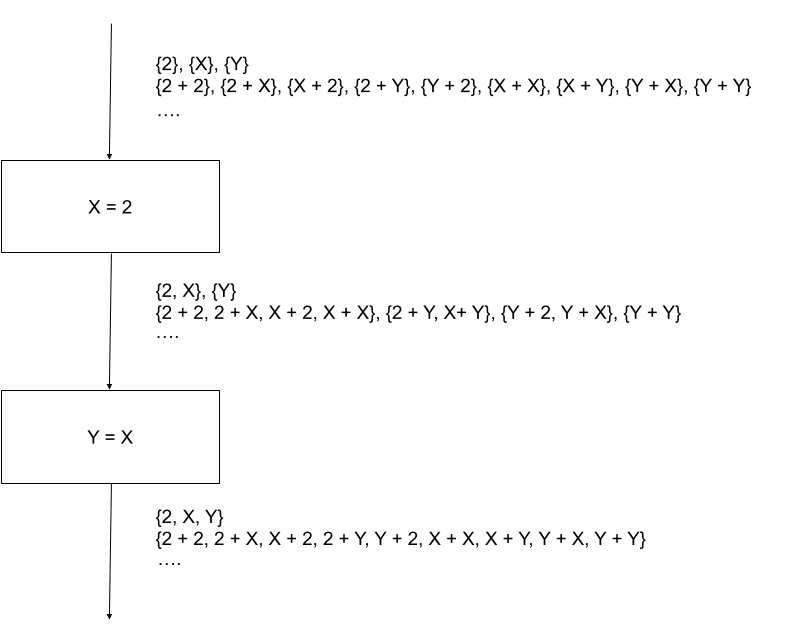
\includegraphics[scale=0.3]{HerbrandEquivalenceTrans.png}
        \caption{Example of Herbrand Equivalence computation at a \textbf{transfer point}}
        \label{fig:herbrandExample}
    \end{figure}
\end{frame}

\begin{frame}{Herbrand Equivalence Computation}
    \begin{figure}[!h]
        \centering
        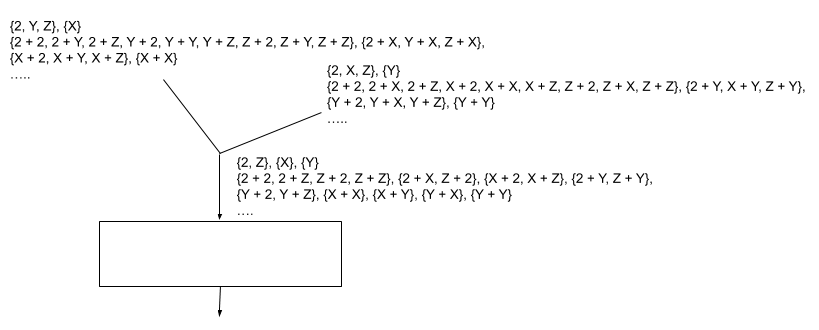
\includegraphics[scale=0.35]{HerbrandEquivalenceConv.png}
        \caption{Example of Herbrand Equivalence computation at a \textbf{confluence point}}
        \label{fig:herbrandExample}
    \end{figure}
\end{frame}

\begin{frame}{Herbrand Equivalence Computation}
    \begin{figure}[!h]
        \centering
        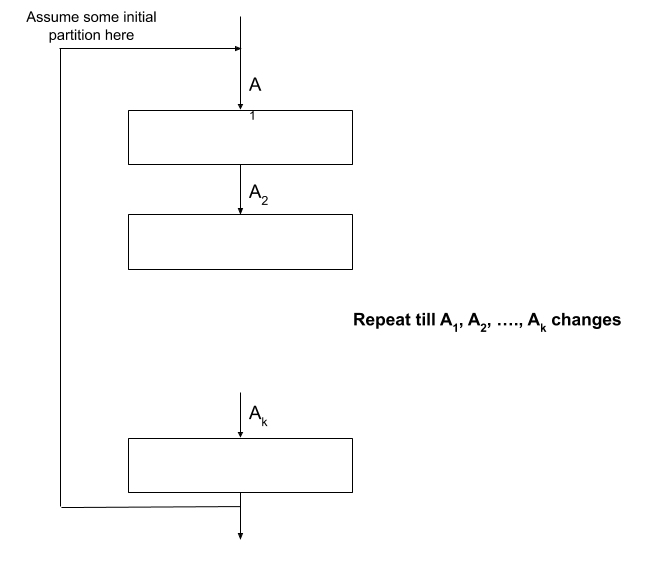
\includegraphics[scale=0.3]{HerbrandEquivalenceLoop.png}
        \caption{Example of Herbrand Equivalence computation in presence of a loop in the program graph}
        \label{fig:herbrandExample}
    \end{figure}
\end{frame}

\begin{frame}{Learning outcome and Challanges faced}
    \textbf{Learnings}
    \begin{itemize}
        \item Working with LLVM
    \end{itemize}
    \textbf{Challanges faced}
    \begin{itemize}
        \item Working with LLVM - there is documentation, but difficult to understand for someone who is new to it
        \item Testing and debugging
    \end{itemize}
\end{frame}

\begin{frame}{References}
\bibliographystyle{IEEEtran}
\bibliography{btp}
\end{frame}

\end{document}